
\begin{frame}[plain,c]
\begin{center}
{\Huge \bf Optional reading for Lecture \thislecture}
\end{center}
\end{frame}

% ------------------------------------------------------------------------------

%
% Worked example :
%

{
\problemslide

%
%
%

\begin{frame}{Worked example: System of 3 wires}

  \begin{blockexmplque}{Question}
    \begin{minipage}[r]{0.75\textwidth}
      Consider 3 straight, infinitely long, coplanar,
      equally spaced wires with zero radius,
      each carrying a current $I$ in the same direction.
      \begin{enumerate}
        \item Find the positions where the magnetic field is zero.
        \item Sketch the magnetic field lines.
        \item If the middle wire is displaced a very small distance $x$
         ($x << d$) to the right (as shown in the diagram)
         while the other 2 wires are held fixed,
         show that it will excecute a simple harmonic oscillation.
         If the wire has linear mass density $\lambda$ (mass per unit length)
         find the angular frequency of oscillation.
      \end{enumerate}
    \end{minipage}
    \begin{minipage}[l]{0.20\textwidth}
     \begin{center}
       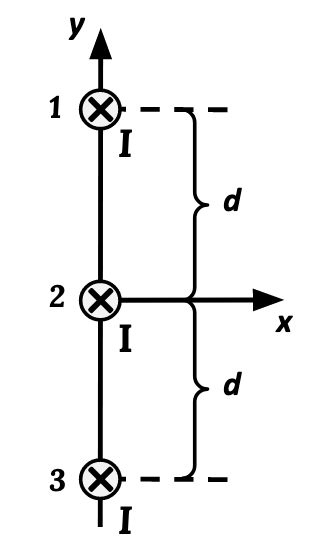
\includegraphics[width=0.94\textwidth]{./images/problems/lect06_3wires_1}
     \end{center}
    \end{minipage}
  \end{blockexmplque}

\end{frame}

%
%
%

\begin{frame}{Worked example: System of 3 wires}

  The magnetic field $\vec{B}$, produced by each long straight wire
  carrying a current $I$, it is azimuthal, and it is given by
  \begin{equation*}
    \vec{B} = \frac{\mu_0 I}{2 \pi r} \hat{\phi}
  \end{equation*}
  where $r$ is the distance from the wire.\\
  \vspace{0.2cm}

  Since the three wires are coplanar, and they carry current in the same direction
  producing similar azimulthal magnetic fields,
  the points of zero magnetic field must be
  located between the wires, and be on the same plane as the wires.
  There must be two zero-field points on each plane perpendicular to the three wires.
  On each such plane, the zero-field points are between the wires and lie on the
  axis that connects the wires.\\
  \vspace{0.2cm}

  Let $y$ be the distance between the middle wire and one of the zero-field points.
  For each such point, the field from the closest
  wire that lies on one side will cancel out the anti-parallel fields from the
  other two wires that lie on the opposite side.

\end{frame}

%
%
%

\begin{frame}{Worked example: System of 3 wires}

  Therefore, we can write:
  \begin{equation*}
      \frac{\mu_0 I}{2\pi(d-y)} = \frac{\mu_0 I}{2\pi y} + \frac{\mu_0 I}{2\pi(d+y)}
  \end{equation*}

  \begin{minipage}[r]{0.55\textwidth}
    The above yields:
    \begin{equation*}
        \frac{1}{d-y} = \frac{1}{y} + \frac{1}{d+y} \Rightarrow
    \end{equation*}
    \begin{equation*}
        \frac{1}{d-y} = \frac{d+2y}{y(d-y)} \Rightarrow
    \end{equation*}
    \begin{equation*}
        y(d+y) = (d-y)(d+2y) \Rightarrow
    \end{equation*}
    \begin{equation*}
        \cancel{yd} + y^2 = d^2 + \cancel{2yd} - \cancel{yd} - 2y^2 \Rightarrow
    \end{equation*}
    \begin{equation*}
        3y^2 = d^2 \Rightarrow
    \end{equation*}
    \begin{equation*}
        y = \pm \frac{d}{\sqrt{3}}
        \label{eq:p3_yvalues_zeroB}
    \end{equation*}
  \end{minipage}
  \begin{minipage}[l]{0.40\textwidth}
    The magnetic field lines, are shown below:
    \begin{center}
      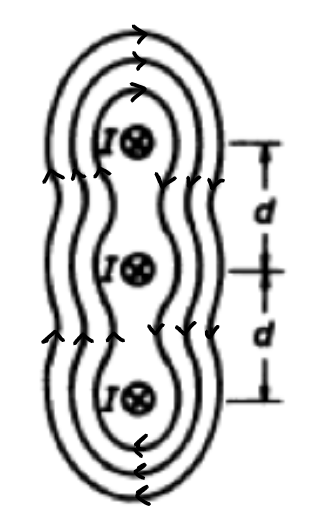
\includegraphics[width=0.50\textwidth]{./images/problems/lect06_3wires_sol_a_1}
    \end{center}
  \end{minipage}

\end{frame}

%
%
%

\begin{frame}{Worked example: System of 3 wires}

  \begin{columns}
    \begin{column}{0.40\textwidth}
      If the middle wire (2) is displaced by a small distance $x$ in the direction of
      the positive $x$ axis, the (attractive) forces $\vec{F}_{21}$ and $\vec{F}_{23}$
      exerted on wire 2 because of wires 1 and 3, correspondingly, are shown in
      the figure on the right.
    \end{column}
    \begin{column}{0.60\textwidth}
      \begin{center}
        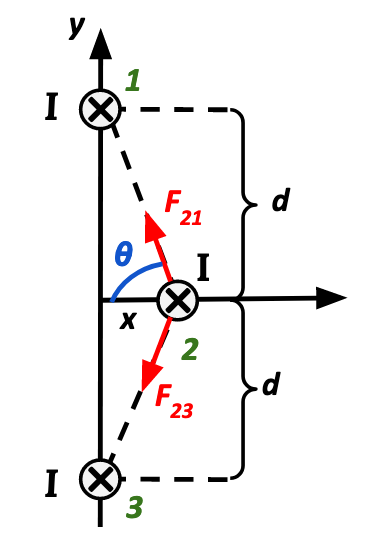
\includegraphics[width=0.70\textwidth]{./images/problems/lect06_3wires_sol_b_1}
      \end{center}
    \end{column}
  \end{columns}

\end{frame}

%
%
%

\begin{frame}{Worked example: System of 3 wires}

  These forces will have the same magnitude, which given by:
  \begin{equation*}
      F_{21} = F_{23} = \frac{\mu_0 I^2}{2\pi \sqrt{d^2+x^2}} L
  \end{equation*}
  where $L$ is the length of the wires.

  As it can be seen, the $y$ components of $\vec{F}_{21}$ and $\vec{F}_{23}$
  cancel out. The (negative) $x$ components of both of these forces
  will contribute to the total force $\vec{F}_{2}$ exerted on wire 2,
  which is given by:
  \begin{equation*}
      \vec{F}_2 = - \Big( F_{21} cos\theta + F_{23} cos\theta \Big) \hat{x}
  \end{equation*}

  Using the expressions we derived for $F_{21}$ and $F_{23}$,
  the above becomes:
  \begin{equation*}
      \vec{F}_2 = - \cancel{2} \frac{\mu_0 I^2}{\cancel{2}\pi \sqrt{d^2+x^2}} L cos\theta \hat{x}
  \end{equation*}

\end{frame}

%
%
%

\begin{frame}{Worked example: System of 3 wires}

  Given that:
  \begin{equation*}
      cos\theta = \frac{x}{\sqrt{d^2+x^2}}
  \end{equation*}
  the previous expression for $\vec{F}_2$ can be written as:
  \begin{equation*}
      \vec{F}_2 = - \frac{\mu_0 I^2}{\pi} \frac{x}{d^2+x^2} L \hat{x} \xRightarrow{d^2+x^2 \approx d^2}
  \end{equation*}

  \begin{equation*}
      \vec{F}_2 = - \frac{\mu_0 I^2 L}{\pi d^2} x \hat{x}
  \end{equation*}

  As it can be seen, the force is proportional and opposite to the
  displacement, Hence the motion of the wire is a simple harmonic oscillation
  about the equilibrium position at $x$=0.

  Using Newton's second law, we can write:
  \begin{equation*}
      \vec{F}_2 = m \frac{d^2 x}{dt^2} \hat{x} \Rightarrow
  \end{equation*}

\end{frame}

%
%
%

\begin{frame}{Worked example: System of 3 wires}

  \begin{equation*}
      - \frac{\mu_0 I^2 L}{\pi d^2} x \hat{x} = m \frac{d^2 x}{dt^2} \hat{x}
      \xRightarrow{m = \lambda L}
  \end{equation*}

  \begin{equation*}
      - \frac{\mu_0 I^2 L}{\pi d^2} x = \lambda L \frac{d^2 x}{dt^2} \Rightarrow
  \end{equation*}

  \begin{equation*}
     \frac{d^2 x}{dt^2} + \frac{\mu_0 I^2}{\pi \lambda d^2} x
  \end{equation*}

  which has the form of the known equation of
  motion for a harmonic oscillator (\"x+$\omega^2$x = 0).
  From this we can deduce that the angular frequency of oscillation, $\omega$,
  is given by:

  \begin{equation*}
     \omega = \sqrt{\frac{\mu_0 I^2}{\pi \lambda d^2}} =
      \frac{I}{d} \sqrt{\frac{\mu_0}{\pi \lambda}}
  \end{equation*}

\end{frame}

} % Worked example

% ------------------------------------------------------------------------------
